\section{Resumen}
El acceso a herramientas de gestión energética accesibles sigue siendo limitado en Colombia debido a los altos costos de las soluciones tradicionales, lo que afecta especialmente a los usuarios de consumo medio y bajo. En este contexto, las tecnologías de Internet de las Cosas (IoT) surgen como una opción innovadora y de bajo costo que permite recopilar, transmitir y procesar información en tiempo real, facilitando un mayor control sobre el uso de la energía.
Este trabajo tiene como propósito analizar la factibilidad y los beneficios de un sistema de gestión de información energética basado en IoT, tomando como referencia la propuesta de Vatia S.A. E.S.P. El estudio busca demostrar cómo la implementación de estas tecnologías puede facilitar la eficiencia energética y ampliar el acceso a prácticas de gestión en sectores donde usualmente no se aplican. Al ofrecer alternativas de bajo costo y fácil implementación, los sistemas IoT no solo promueven un uso más racional de la energía, sino que también contribuyen a mejorar la competitividad del mercado eléctrico colombiano y a fortalecer la sostenibilidad y modernización del sistema energético nacional.

\section{Introducción}
El sostenido crecimiento en la demanda eléctrica de Colombia, impulsado por desarrollo económico y demográfico plantea un desafío crítico para la sostenibilidad y competitividad del sistema energético nacional, lo cual exige la incorporación de herramientas que permitan a los usuarios conocer y gestionar su consumo, pero se sabe que la mayoría de las soluciones disponibles en el mercado suelen tener costos elevados, lo que limita el acceso a los usuarios con consumos más bajos, precisamente aquellos que representan una gran parte del sistema eléctrico nacional.  
\newline
Ante esta situación, las tecnologías asociadas al internet de las cosas (IOT) surgen como una alternativa para desarrollar sistemas de control y monitoreo más accesibles, debido a que estos recopilan, transmiten y procesan información eléctrica en tiempo real, lo cual facilita observar los consumos y datos en distintas interfaces. Al ser soluciones de bajo costo resultan muy beneficiosas para impulsar la masificación de la gestión energética en sectores donde no se implementan estos tipos de prácticas.  
\newline
Este trabajo tiene como propósito analizar la factibilidad y los beneficios de un sistema de gestión de información energética basado en tecnologías IoT, tomando como caso la propuesta de Vatia S.A. E.S.P. El estudio se enfoca en usuarios de consumo medio y bajo, con el fin de evaluar cómo estas soluciones pueden facilitar la eficiencia energética, mejorar la competitividad del mercado eléctrico colombiano y facilitar el acceso a herramientas de gestión.

Ante esta situación, las tecnologías asociadas al Internet de las Cosas (IoT) surgen como una alternativa para desarrollar sistemas de control y monitoreo más accesibles, debido a que estos recopilan, transmiten y procesan información eléctrica en tiempo real, lo cual facilita la observación de los consumos y datos en distintas interfaces. Al ser soluciones de bajo costo, resultan muy beneficiosas para impulsar la masificación de la gestión energética en sectores donde no se implementan este tipo de prácticas.

Este trabajo tiene como propósito analizar la factibilidad y los beneficios de un sistema de gestión de información energética basado en tecnologías IoT, tomando como caso la propuesta de Vatia S.A. E.S.P. \cite{Jaramillo2022}. El estudio se enfoca en usuarios de consumo medio y bajo, con el fin de evaluar cómo estas soluciones pueden facilitar la eficiencia energética, mejorar la competitividad del mercado eléctrico colombiano y facilitar el acceso a herramientas de gestión.

\section{¿Qué es IoT?}
El Internet de las Cosas (IoT) se refiere a un paradigma tecnológico que permite la interconexión de dispositivos y objetos a través de Internet, facilitando la comunicación y el intercambio de datos entre ellos. Este concepto ha evolucionado de ser una mera idea académica a convertirse en un ecosistema con aplicaciones industriales y comerciales significativas, que tienen implicaciones tecnológicas y sociales importantes \cite{MoralesTamayoYoandrys2025AdId}.

El IoT se basa en la colaboración entre sensores inteligentes que realizan tareas de manera autónoma, sin necesidad de intervención humana. Esto se traduce en la capacidad de recolectar, analizar y monitorear datos en tiempo real, lo que resulta en mejoras en la eficiencia operativa y la sostenibilidad en diversos sectores, como la industria electromecánica y la gestión energética en entornos residenciales y universitarios \cite{OlivaresGorritiEneko2022Eydd}, \cite{RomeroMacíasJavierVidal2025Adid}.
Por ejemplo, en la industria electromecánica, se ha observado que las aplicaciones de IoT pueden optimizar el mantenimiento predictivo, la gestión energética y la gestión de inventarios, contribuyendo a la reducción de costos y emisiones.


\section{Implementación}
Para llevar a cabo la implementación del sistema de monitoreo y control automático, se arrancó con una etapa de pruebas básicas en laboratorio. Ahí se verificó que los equipos de comunicación diseñados localmente funcionaran bien con los medidores de energía, revisando voltajes, estabilidad y que los datos viajaran sin problema \cite{Jaramillo2022}.


\begin{figure}[h!]
\centering
\includegraphics[width=0.48\textwidth]{figs/Visualización del PCB y equipo celular ensamblado en la caja pag15.png}
\caption{Visualización del PCB y equipo celular ensamblado en la caja. imagen extraída de \cite[pag.~15]{Jaramillo2022}.}
\label{fig:factura3}
\end{figure}

Una vez superado ese filtro, se pasó a pruebas en campo con clientes en distintas ciudades del país, lo que permitió comprobar que el sistema operaba en condiciones reales usando redes celulares, Ethernet y también enlaces de radiofrecuencia.

\begin{figure}[h!]
\centering
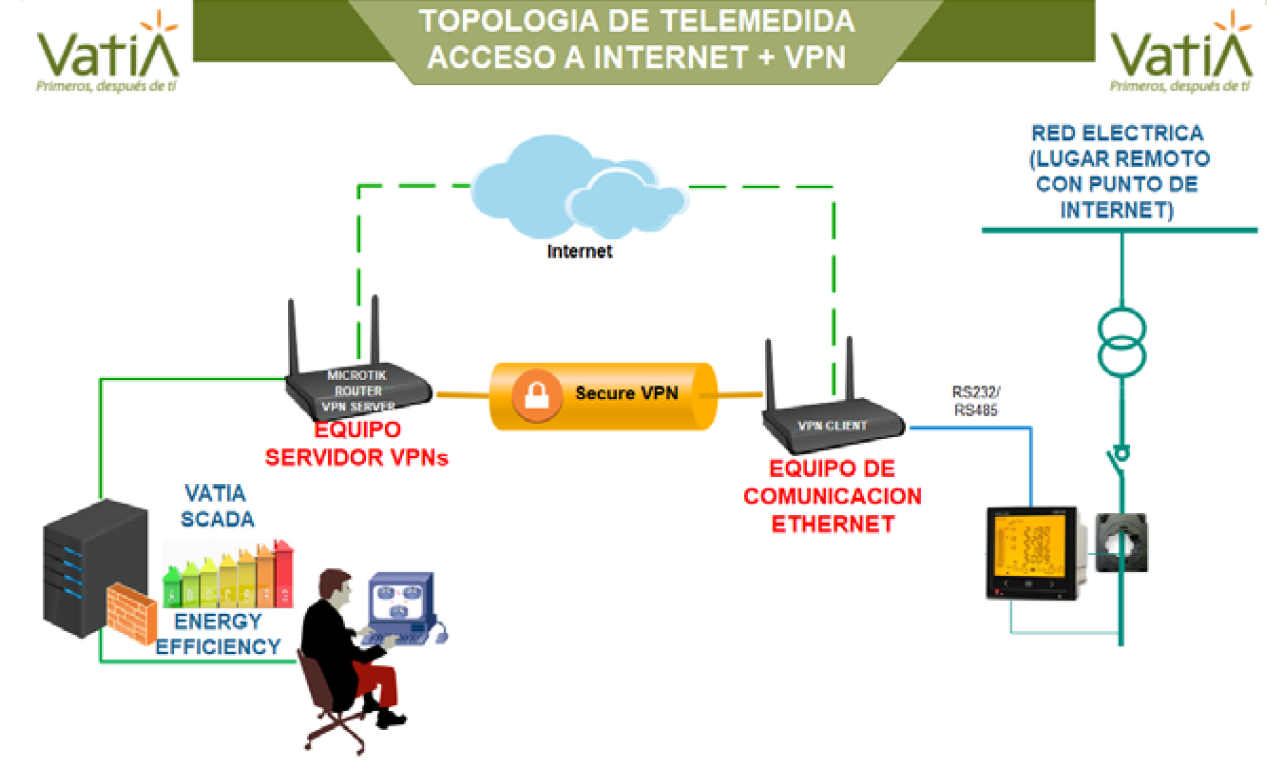
\includegraphics[width=0.48\textwidth]{figs/Topología de telemedida a través de un equipo Ethernet con acceso a internet pag 12.png}
\caption{Topología de telemedida a través de un equipo Ethernet con acceso a internet. imagen extraída de \cite[pag.~12]{Jaramillo2022}.}
\label{fig:factura1}
\end{figure}

Durante el proceso se usaron plataformas de gestión tipo SCADA, que facilitaron la integración de variables eléctricas con otra información de interés para cada usuario. Todo esto se hizo bajo la lógica de producto viable, es decir, se sacaban versiones sencillas, se probaban con usuarios y, a partir de su opinión, se ajustaba el diseño. Gracias a ese método, el sistema tomó forma, llegando así a una versión más completa y estable.

El sistema no solo permite medir y visualizar, sino que también ofrece herramientas como la proyección del gasto energético, simulación de facturas y reportes de calidad eléctrica. Con estas funciones, los clientes pueden identificar cuándo tomar decisiones para reducir sus costos energéticos.

\begin{figure}[h!]
\centering
\includegraphics[width=0.48\textwidth]{figs/Visualización de las herramientas desarrolladas pag 8.png}
\caption{Visualización de las herramientas desarrolladas. imagen extraída de \cite[pag.~8]{Jaramillo2022}.}
\label{fig:factura2}
\end{figure}

\begin{figure}[h!]
\centering
\includegraphics[width=0.48\textwidth]{figs/Pantalla de Herramienta de simulación de factura desarrollada pag 9.png}
\caption{Pantalla de la herramienta de simulación de facturas desarrollada por la empresa Vatia. imagen extraída de \cite[pag.~9]{Jaramillo2022}.}
\label{fig:factura}
\end{figure}

\begin{figure}[h!]
\centering
\includegraphics[width=0.48\textwidth]{figs/Pantalla de la herramienta de calidad de energía pag 10.png}
\caption{Pantalla de la herramienta de simulación de facturas desarrollada por la empresa Vatia. imagen extraída de \cite[pag.~10]{Jaramillo2022}.}
\label{fig:factura0}
\end{figure}

Ya en la etapa comercial, se instalaron equipos en sectores como industrias y instituciones educativas, lo cual demostró que la solución es escalable y se adapta a distintas necesidades. Además, el uso de tecnologías IoT de bajo costo hizo posible que usuarios con consumos medios o bajos —quienes usualyacceden a este tipo de herramientas por lo costoso de los equipos importados— pudieran contar con una solución efectiva y ajustada a sus realidades.

En resumen, la implementación dejó claro que sí es posible combinar innovación, economía y cumplimiento normativo para entregar un sistema confiable, sostenible y capaz de integrar servicios adicionales en el futuro, fortaleciendo así la eficiencia energética y la competitividad de las empresas en el contexto colombiano \cite{Jaramillo2022}.

\section{Beneficios}
La principal ventaja de este sistema es que reduce la barrera de acceso a la eficiencia energética. Antes, solo las empresas grandes podían pagar equipos importados para medir y controlar el consumo; ahora, con la solución desarrollada localmente por Vatia \cite{Jaramillo2022}, los costos bajan y hasta negocios pequeños o instituciones con consumos moderados pueden usarla sin problema.

Otro beneficio clave es el ahorro económico. Como los dispositivos son locales, no hay que gastar en importaciones y, además, se ajustan mejor a las condiciones del país. Encima, la plataforma muestra en tiempo real el gasto y hasta simula facturas, lo que ayuda a gestionar los gastos y a evitar sorpresas en la factura.

También se obtiene una mejora en la organización y competitividad. Tener datos claros del consumo permite que las empresas tomen decisiones rápidas, como apagar lo que no se está usando, mejorar procesos o evitar pérdidas de energía. Eso, al final, se traduce en menos costos y más productividad.

El sistema no se queda solo en medir voltajes o corrientes. Se puede conectar con otras variables como temperatura o humedad, lo que lo hace útil para muchos sectores: agricultura, comercio, industria o cualquier negocio que dependa de varias condiciones al mismo tiempo. Y, por supuesto, el tema ambiental es muy importante. Al consumir la energía de manera más eficaz, se reduce el desperdicio y, con eso, también el impacto negativo en el medio ambiente. Esto es un beneficio doble porque se ahorra dinero y se protege el planeta.



\section*{Tabla IoT - Sistema de Monitoreo y Control Automático}
Observese el cuadro \ref{tab:table}. 
\begin{table*}[t!]
\centering
\caption{Tabla IoT - Sistema de Monitoreo y Control Automático}
\label{tab:table}
\begin{tabular}{@{}p{3.5cm}p{6cm}p{6cm}@{}}
\toprule
\textbf{Aspecto} & \textbf{Descripción} & \textbf{Ejemplo del proyecto} \\
\midrule
Plataforma en línea & Permite lectura, visualización, control y administración energética en tiempo real. & SCADA para gestión de energía y multiusuario. \\
\addlinespace
Sistemas de medida & Analizadores de red, transformadores de corriente y voltaje. Integración con fuentes adicionales vía Modbus, REST, MQTT, SQL. & CVM-C5, CVM-C10, medidores Elster e Itron. \\
\addlinespace
Herramientas de gestión & Incluyen proyección de consumos, simulación de facturas, alertas automáticas, informes y monitoreo de calidad de energía. & Pantallas de consumo, semáforos de calidad, facturación simulada. \\
\addlinespace
Dispositivos de comunicación & Equipos de bajo costo desarrollados localmente: celular, Ethernet y radiofrecuencia (LORA). & Dispositivo celular 2G/3G/4G con interfaz serial RS485. \\
\addlinespace
Topologías de comunicación & Se adaptan según cobertura: celular, red Ethernet o radiofrecuencia de largo alcance. & Equipo Ethernet con VPN o red celular en sótanos con RF. \\
\addlinespace
Beneficios & Bajo costo, escalabilidad, integración de nuevos servicios IoT, competitividad para usuarios finales. & Monitoreo en zoológico y en hidroeléctrica con medidores de distintas marcas. \\
\addlinespace
Aplicaciones adicionales & Monitoreo y control de variables no eléctricas que afectan procesos productivos. & Temperatura en cadenas de frío, humedad en sistemas agrícolas. \\
\bottomrule
\end{tabular}
\end{table*}

\section{Conclusiones}

El proyecto de Vatia S.A. E.S.P. resalta cómo el IoT puede transformar la vida de las personas en Colombia. Gracias a su bajo costo, ahora usuarios de diferentes niveles socioeconómicos pueden gestionar su consumo energético de manera más efectiva. Si esta tecnología se vuelve común, podría integrarse con la domótica, permitiendo no solo la supervisión, sino también la implementación de acciones concretas para ahorrar energía. Esto sería un paso fundamental: pasar de recopilar datos a tomar decisiones que realmente impacten el día a día de las personas.